
\chapter{Funciones fructíferas }

\label{funcReturn}

\section{Valores de retorno}

\index{valor de retorno}

Algunas de las funciones primitivas que hemos usado, como las matemáticas,
entregan resultados. El llamar a estas funciones genera un valor nuevo,
que usualmente asignamos a una variable o usamos como parte de una
expresión.\inputencoding{latin9}
\begin{lstlisting}
e = math.exp(1.0)
altura = radio * math.sin(angulo)
\end{lstlisting}
\inputencoding{utf8}
Pero hasta ahora ninguna de las funciones que hemos escrito ha retornado
un valor.

En este capítulo vamos a escribir funciones que retornan valores,
los cuales denominamos \textbf{funciones fructíferas}, o provechosas\footnote{En algunos libros de programación, las \textit{funciones} que desarrollamos
en el capítulo anterior se denominan \textit{procedimientos} y las
que veremos en este capítulo sí se denominan \textit{funciones}, ya
que los lenguajes de programación usados para enseñar (como Pascal)
hacían la distinción. Muchos lenguajes de programación vigentes (incluido
Python y C) no diferencian sintácticamente entre procedimientos y
funciones, por eso usamos esta terminología.}. El primer ejemplo es \texttt{area}, que retorna el área de un círculo
dado su radio:\inputencoding{latin9}
\begin{lstlisting}
import math

def area(radio):
  temp = math.pi * radio**2
  return temp
\end{lstlisting}
\inputencoding{utf8}
Ya nos habíamos topado con la sentencia \texttt{return} antes, pero,
en una función fructífera, la sentencia \texttt{return} incluye un
\textbf{valor de retorno}. Esta sentencia significa: ``Retorne inmediatamente
de esta función y use la siguiente expresión como un valor de retorno.''
La expresión proporcionada puede ser arbitrariamente compleja, así
que podríamos escribir esta función más concisamente:

\inputencoding{latin9}\begin{lstlisting}
def area(radio):
  return math.pi * radio**2
\end{lstlisting}
\inputencoding{utf8} 

Por otro lado, las \textbf{variables temporales}, como \texttt{temp},
a menudo permiten depurar los programas más fácilmente.

\index{variable temporal} \index{variable!temporal}

Algunas veces es muy útil tener múltiples sentencias return, ubicadas
en ramas distintas de un condicional:

\inputencoding{latin9}\begin{lstlisting}
def valorAbsoluto(x):
  if x < 0:
    return -x
  else:
    return x
\end{lstlisting}
\inputencoding{utf8}
Ya que estas sentencias \texttt{return} están en un condicional alternativo,
sólo una será ejecutada. Tan pronto como esto suceda, la función termina
sin ejecutar las sentencias que siguen.

El código que aparece después de la sentencia \texttt{return}, o en
un lugar que el flujo de ejecución nunca puede alcanzar, se denomina
\textbf{código muerto}.

\index{código muerto}

En una función fructífera es una buena idea garantizar que toda ruta
posible de ejecución del programa llegue a una sentencia \texttt{return}.
Por ejemplo:

\inputencoding{latin9}\begin{lstlisting}
def valorAbsoluto(x):
  if x < 0:
    return -x
  elif x > 0:
    return x
\end{lstlisting}
\inputencoding{utf8} Este programa no es correcto porque si \texttt{x} llega a ser 0,
ninguna condición es cierta y la función puede terminar sin alcanzar
una sentencia \texttt{return}. En este caso el valor de retorno que
Python entrega es un valor especial denominado \texttt{None}:

\index{None}\inputencoding{latin9}
\begin{lstlisting}
>>> print(valorAbsoluto(0))
None
\end{lstlisting}
\inputencoding{utf8}
\section{Desarrollo de programas}

\label{program development} \index{andamiaje}

En este momento usted debería ser capaz de leer funciones completas
y deducir lo que hacen. También, si ha realizado los ejercicios, ya
ha escrito algunas funciones pequeñas. A medida en que usted escriba
funciones más grandes puede empezar a tener una dificultad mayor,
especialmente con los errores semánticos y de tiempo de ejecución.

Para desarrollar programas cada vez más complejos, vamos a sugerir
una técnica denominada \textbf{desarrollo incremental}. El objetivo
del desarrollo incremental es evitar largas sesiones de depuración
mediante la adición y prueba de una pequeña cantidad de código en
cada paso.

\index{desarrollo incremental} \index{desarrollo!incremental}

Como ejemplo, suponga que usted desea hallar la distancia entre dos
puntos dados por las coordenadas $(x_{1},y_{1})$ y $(x_{2},y_{2})$.
Por el teorema de Pitágoras, la distancia se calcula con:

\begin{equation}
distancia=\sqrt{(x_{2}-x_{1})^{2}+(y_{2}-y_{1})^{2}}
\end{equation}
El primer paso es considerar cómo luciría la función \texttt{distancia}
en Python. En otras palabras, ¿cuales son las entradas (parámetros)
y cual es la salida (valor de retorno)?

En este caso, los dos puntos son las entradas, que podemos representar
usando cuatro parámetros. El valor de retorno es la distancia, que
es un valor de punto flotante.

Ya podemos escribir un borrador de la función:

\inputencoding{latin9}\begin{lstlisting}
def distancia(x1, y1, x2, y2):
  return 0.0
\end{lstlisting}
\inputencoding{utf8} Obviamente, esta versión de la función no calcula distancias; siempre
retorna cero. Pero es correcta sintácticamente y puede correr, lo
que implica que la podemos probar antes de que la hagamos más compleja.

Para probar la nueva función la llamamos con valores simples:

\inputencoding{latin9}\begin{lstlisting}
>>> distancia(1, 2, 4, 6)
0.0
\end{lstlisting}
\inputencoding{utf8} Escogemos estos valores de forma que la distancia horizontal sea
3 y la vertical 4; de esta forma el resultado es 5 (la hipotenusa
de un triángulo con medidas 3-4-5). Cuando probamos una función es
fundamental conocer algunas respuestas correctas.

En este punto hemos confirmado que la función está bien sintácticamente,
y que podemos empezar a agregar líneas de código. Después de cada
cambio, probamos la función otra vez. Si hay un error, sabemos dónde
debe estar —en la última línea que agregamos.

Un primer paso lógico en este cómputo es encontrar las diferencias
$x_{2}-x_{1}$ y $y_{2}-y_{1}$. Almacenaremos estos valores en variables
temporales llamadas \texttt{dx} y \texttt{dy} y los imprimiremos.

\inputencoding{latin9}\begin{lstlisting}
def distancia(x1, y1, x2, y2):
  dx = x2 - x1
  dy = y2 - y1
  print("dx es", dx)
  print("dy es", dy)
  return 0.0
\end{lstlisting}
\inputencoding{utf8} Si la función trabaja bien, las salidas deben ser 3 y 4. Si es así,
sabemos que la función está obteniendo los parámetros correctos y
calculando el primer paso correctamente. Si no ocurre ésto, entonces
hay unas pocas líneas para chequear.

Ahora calculamos la suma de los cuadrados de \texttt{dx} y \texttt{dy}:

\inputencoding{latin9}\begin{lstlisting}
def distancia(x1, y1, x2, y2):
  dx = x2 - x1
  dy = y2 - y1
  discuadrado = dx**2 + dy**2
  print("discuadrado es: ", discuadrado)
  return 0.0
\end{lstlisting}
\inputencoding{utf8} Note que hemos eliminado las sentencias \texttt{print} que teníamos
en el paso anterior. Este código se denomina \textbf{andamiaje} porque
es útil para construir el programa pero no hace parte del producto
final.

De nuevo, corremos el programa y chequeamos la salida (que debe ser
25).

Finalmente, si importamos el módulo math, podemos usar la función
\texttt{sqrt} para calcular y retornar el resultado:

\inputencoding{latin9}\begin{lstlisting}
def distancia(x1, y1, x2, y2):
  dx = x2 - x1
  dy = y2 - y1
  discuadrado = dx**2 + dy**2
  resultado = math.sqrt(discuadrado)
  return resultado
\end{lstlisting}
\inputencoding{utf8} Si esto funciona bien, usted ha terminado. Si no, se podría imprimir
el valor de \texttt{resultado} antes de la sentencia return.

Recapitulando, para empezar, usted debería agregar solamente una línea
o dos cada vez.

A medida que gane más experiencia podrá escribir y depurar trozos
mayores. De cualquier forma el proceso de desarrollo incremental puede
evitarle mucho tiempo de depuración.

Los aspectos claves del proceso son:
\begin{enumerate}
\item Empezar con un programa correcto y hacer pequeños cambios incrementales.
Si en cualquier punto hay un error, usted sabrá exactamente donde
está.
\item Use variables temporales para almacenar valores intermedios de manera
que se puedan imprimir y chequear.
\item Ya que el programa esté corriendo, usted puede remover parte del andamiaje
o consolidar múltiples sentencias en expresiones compuestas, pero
sólo si esto no dificulta la lectura del programa.
\end{enumerate}

\section{Composición}

\index{composición} \index{función!composición}

Como usted esperaría, se puede llamar una función fructífera desde
otra. Esta capacidad es la \textbf{composición}.

Como ejemplo vamos a escribir una función que toma dos puntos: el
centro de un círculo y un punto en el perímetro, y que calcule el
área total del círculo.

Asuma que el punto central está almacenado en las variables \texttt{xc}
y \texttt{yc}, y que el punto perimetral está en \texttt{xp} y \texttt{yp}.
El primer paso es encontrar el radio del círculo, que es la distancia
entre los dos puntos. Afortunadamente, hay una función, \texttt{distancia},
que hace eso:

\inputencoding{latin9}\begin{lstlisting}
radio = distancia(xc, yc, xp, yp)
\end{lstlisting}
\inputencoding{utf8}
El segundo paso es encontrar el área de un círculo con dicho radio
y retornarla:

\inputencoding{latin9}\begin{lstlisting}
resultado = area(radio)
return resultado
\end{lstlisting}
\inputencoding{utf8} Envolviendo todo en una función obtenemos:

\inputencoding{latin9}\begin{lstlisting}
def area2(xc, yc, xp, yp):
  radio = distancia(xc, yc, xp, yp)
  resultado = area(radio)
  return resultado
\end{lstlisting}
\inputencoding{utf8}Llamamos a esta función \texttt{area2} para distinguirla de la función
\texttt{area} definida previamente. Solo puede haber una función con
un nombre dado dentro de un módulo.

Las variables temporales \texttt{radio} y \texttt{area} son útiles
para desarrollar y depurar, pero una vez que el programa está funcionando
podemos hacer la función más concisa componiendo las llamadas a funciones:

\inputencoding{latin9}\begin{lstlisting}
def area2(xc, yc, xp, yp):
  return area(distancia(xc, yc, xp, yp))
\end{lstlisting}
\inputencoding{utf8}
\section{Funciones booleanas}

\label{boolean} \index{función booleana} \index{función booleana}

Las funciones que pueden retornar un valor booleano son convenientes
para ocultar chequeos complicados adentro de funciones. Por ejemplo:

\inputencoding{latin9}\begin{lstlisting}
def esDivisible(x, y):
  if x % y == 0:
    return True       #  es cierto
  else:
    return False      # es falso
\end{lstlisting}
\inputencoding{utf8} El nombre de esta función es \texttt{esDivisible}. Es muy usual nombrar
las funciones booleanas con palabras o frases que suenan como preguntas
de sí o no (que tienen como respuesta un sí o un no). \texttt{esDivisible}
retorna \texttt{True} ó \texttt{False} para indicar si x es divisible
exactamente por y.

Podemos hacerla más concisa tomando ventaja del hecho de que una condición
dentro de una sentencia \texttt{if} es una expresión booleana. Podemos
retornarla directamente, evitando completamente el \texttt{if}:

\inputencoding{latin9}\begin{lstlisting}
def esDivisible(x, y):
  return x % y == 0
\end{lstlisting}
\inputencoding{utf8} Esta sesión muestra la nueva función en acción:

\inputencoding{latin9}\begin{lstlisting}
>>>   esDivisible(6, 4)
False
>>>   esDivisible(6, 3)
True
\end{lstlisting}
\inputencoding{utf8}
Las funciones booleanas se usan a menudo en las sentencias condicionales:

\inputencoding{latin9}\begin{lstlisting}
if esDivisible(x, y):
  print("x es divisible por y")
else:
  print("x no es divisible por y")
\end{lstlisting}
\inputencoding{utf8} Puede parecer tentador escribir algo como:

\inputencoding{latin9}\begin{lstlisting}
if esDivisible(x, y) == True:
\end{lstlisting}
\inputencoding{utf8} Pero la comparación extra es innecesaria.

\section{Más recursión}

\index{recursión} \index{lenguaje completo} \index{lenguaje!completo}
\index{Turing, Alan} \index{Turing, Tésis de}

Hasta aquí, usted sólo ha aprendido un pequeño subconjunto de Python,
pero podría interesarle saber que este subconjunto es un lenguaje
de programación {\em completo}, lo que quiere decir que cualquier
cosa que pueda ser calculada puede ser expresada en este subconjunto.
Cualquier programa escrito alguna vez puede ser reescrito usando solamente
las características que usted ha aprendido hasta ahora (de hecho,
necesitaría algunos comandos mas para manejar dispositivos como el
teclado, el ratón, los discos, etc., pero eso sería todo).

Demostrar esta afirmación no es un ejercicio trivial y fue logrado
por Alan Turing, uno de los primeros científicos de la computación
(algunos dirían que el era un matemático, pero la mayoría de los científicos
pioneros de la computación eran matemáticos). Esto se conoce como
la Tesis de Turing. Si usted toma un curso de Teoría de la Computación
tendrá la oportunidad de ver la demostración.

Para darle una idea de lo que puede hacer con las herramientas que
ha aprendido, vamos a evaluar unas pocas funciones matemáticas definidas
recursivamente.

Una definición recursiva es similar a una circular, ya que éstas contienen
una referencia al concepto que se pretende definir. Una definición
circular verdadera no es muy útil:
\begin{description}
\item [{frabjuoso:}] un adjetivo usado para describir algo que es frabjuoso.
\end{description}
\index{frabjuoso} \index{definición circular} \index{definición!circular}

Si usted viera dicha definición en el diccionario, quedaría confundido.
Por otro lado, si encontrara la definición de la función factorial
hallaría algo como esto:

\vspace{-0.35in}
 
\begin{eqnarray*}
 &  & 0!=1\\
 &  & n!=n(n-1)!
\end{eqnarray*}
\vspace{-0.25in}

Esta definición dice que el factorial de 0 es 1, y que el factorial
de cualquier otro valor, $n$, es $n$ multiplicado por el factorial
de $n-1$.

Así que $3!$ es 3 veces $2!$, que es 2 veces $1!$, que es 1 vez
$0!$. Juntando todo esto, $3!$ es igual a 3 veces 2 veces 1 vez
1, lo que da 6.

\index{función factorial} \index{función!factorial}

Si usted puede escribir una definición recursiva para algo, usualmente
podrá escribir un programa para evaluarlo. El primer paso es decidir
cuales son los parámetros para esta función. Con un poco de esfuerzo
usted concluiría que \texttt{factorial} recibe un único parámetro:

\inputencoding{latin9}\begin{lstlisting}
def factorial(n):
\end{lstlisting}
\inputencoding{utf8}
Si el argumento es 0, todo lo que hacemos es retornar 1:

\inputencoding{latin9}\begin{lstlisting}
def factorial(n):
  if n == 0:
    return 1
\end{lstlisting}
\inputencoding{utf8} 

Sino, y ésta es la parte interesante, tenemos que hacer una llamada
recursiva para encontrar el factorial de $n-1$ y, entonces, multiplicarlo
por $n$:\inputencoding{latin9}
\begin{lstlisting}
def factorial(n):
  if n == 0:
    return 1
  else:
    recur = factorial(n-1)
    da = n * recur
    return da
\end{lstlisting}
\inputencoding{utf8}
El flujo de ejecución de este programa es similar al flujo de \texttt{conteo}
en la Sección~\ref{recursion}. Si llamamos a \texttt{factorial}
con el valor 3:

\adjustpage{1}

Como 3 no es 0, tomamos la segunda rama y calculamos el factorial
de \texttt{n-1}...
\begin{quote}
Como 2 no es 0, tomamos la segunda rama y calculamos el factorial
de \texttt{n-1}...

\begin{quote}
Como 1 no es 0, tomamos la segunda rama y calculamos el factorial
de \texttt{n-1}...

\begin{quote}
Como 0 {\em es} 0, tomamos la primera rama y retornamos 1 sin hacer
más llamados recursivos. 
\end{quote}
El valor de retorno (1) se multiplica por $n$, que es 1, y el resultado
se retorna. 
\end{quote}
El valor de retorno (1) se multiplica por $n$, que es 2, y el resultado
se retorna. 
\end{quote}
El valor de retorno (2) se multiplica por $n$, que es 3, y el resultado,
6, se convierte en el valor de retorno del llamado de función que
empezó todo el proceso.

Así queda el diagrama de pila para esta secuencia de llamados de función:

\vspace{0.1in}
 \beforefig \centerline{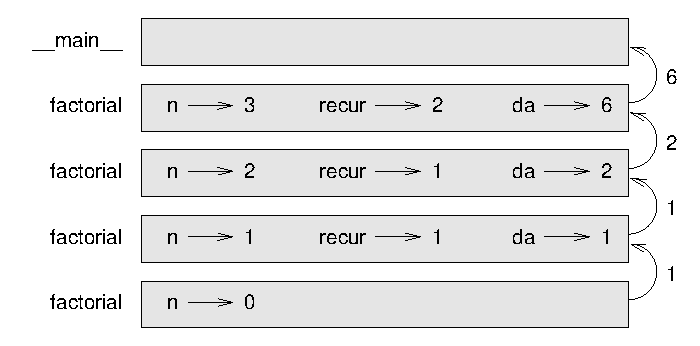
\includegraphics{illustrations/stack3}}
\afterfig \vspace{0.1in}

Los valores de retorno mostrados se pasan hacia arriba a través de
la pila. En cada marco, el valor de retorno es el valor de \texttt{da},
que es el producto de \texttt{n} y \texttt{recur}.

Observe que en el último marco, las variables locales \texttt{recur}
y \texttt{da} no existen porque la rama que las crea no se ejecutó.

\section{El salto de fe}

\index{recursión} \index{salto de fe}

Seguir el flujo de ejecución es una forma de leer programas, pero
rápidamente puede tornarse algo laberíntico. Una alternativa es lo
que denominamos hacer el ``salto de fe.'' Cuando usted llega a un
llamado de función, en lugar de seguir el flujo de ejecución, se {\em
asume} que la función trabaja correctamente y retorna el valor apropiado.

De hecho, usted ya está haciendo el salto de fe cuando usa las funciones
primitivas. Cuando llama a \texttt{math.cos} ó a \texttt{math.exp},
no está examinando las implementaciones de estas funciones. Usted
sólo asume que están correctas porque los que escribieron el módulo
math son buenos programadores.

Lo mismo se cumple para una de sus propias funciones. Por ejemplo,
en la Sección~\ref{boolean}, escribimos una función llamada \texttt{esDivisible}
que determina si un número es divisible por otro. Una vez que nos
hemos convencido de que esta función es correcta —probándola y examinando
el código—podemos usarla sin mirar el código nuevamente.

Lo mismo vale para los programas recursivos. Cuando usted llega a
una llamada recursiva, en lugar de seguir el flujo de ejecución, debería
asumir que el llamado recursivo funciona (retorna el resultado correcto)
y luego preguntarse, ``Asumiendo que puedo encontrar el factorial
de $n-1$, ¿puedo calcular el factorial de $n$?'' En este caso,
es claro que se puede lograr, multiplicándolo por $n$.

Por supuesto que es un poco raro asumir que la función trabaja correctamente
cuando ni siquiera hemos terminado de escribirla, ¡por eso es que
denominamos a esto el salto de fe!.

\section{Un ejemplo más}

\label{one more example}

En el ejemplo anterior usábamos variables temporales para desplegar
los pasos y depurar el código más fácilmente, pero podríamos ahorrar
unas cuantas líneas:

\inputencoding{latin9}\begin{lstlisting}
def factorial(n):
  if n == 0:
    return 1
  else:
    return n * factorial(n-1)
\end{lstlisting}
\inputencoding{utf8} Desde ahora, vamos a usar esta forma más compacta, pero le recomendamos
que use la forma más explícita mientras desarrolla las funciones.
Cuando estén terminadas y funcionando, con un poco de inspiración
se pueden compactar.

\index{La función de Fibonacci}

Después de \texttt{factorial}, el ejemplo más común de función matemática,
definida recursivamente, es la serie de \texttt{fibonacci}, que tiene
la siguiente definición:

\vspace{-0.25in}
 
\begin{eqnarray*}
 &  & fibonacci(0)=1\\
 &  & fibonacci(1)=1\\
 &  & fibonacci(n)=fibonacci(n-1)+fibonacci(n-2);
\end{eqnarray*}
Traducida a Python, luce así:

\inputencoding{latin9}\begin{lstlisting}
def fibonacci (n):
  if n == 0 or n == 1:
    return 1
  else:
    return fibonacci(n-1) + fibonacci(n-2)
\end{lstlisting}
\inputencoding{utf8} Si usted intenta seguir el flujo de ejecución de fibonacci, incluso
para valores pequeños de $n$, le va a doler la cabeza. Pero, si seguimos
el salto de fe, si asumimos que los dos llamados recursivos funcionan
correctamente, es claro que el resultado correcto es la suma de éstos
dos.

\section{Chequeo de tipos}

\index{chequeo de tipos} \index{chequeo de errores} \index{función factorial}

¿Qué pasa si llamamos a \texttt{factorial} y le pasamos a 1.5 como
argumento?

\inputencoding{latin9}\begin{lstlisting}
>>> factorial (1.5)
RuntimeError: Maximum recursion depth exceeded
\end{lstlisting}
\inputencoding{utf8} Parece recursión infinita. ¿Cómo puede darse? Hay un caso base —cuando
\texttt{n == 0}. El problema reside en que los valores de \texttt{n}
se {\em saltan} al caso base .

\index{recursión infinita} \index{recursión!infinita}

En la primera llamada recursiva el valor de \texttt{n} es 0.5. En
la siguiente es -0.5. Desde allí se hace cada vez más pequeño, pero
nunca será 0.

Tenemos dos opciones, podemos intentar generalizar la función \texttt{factorial}
para que trabaje con números de punto flotante, o podemos chequear
el tipo del parámetro que llega. La primera opción se denomina en
matemática la función gama y está fuera del alcance de este libro.
Optaremos por la segunda.

\index{función gama}

Podemos usar la función \texttt{type} para comparar el tipo del parámetro
al tipo de un valor entero conocido (como 1). Mientras estamos en
eso también aseguraremos que el parámetro sea positivo:

\inputencoding{latin9}\begin{lstlisting}
def factorial (n):
  if type(n) != type(1):
    print("Factorial solo esta definido para enteros.")
    return -1
  elif n < 0:
    print("Factorial solo esta definido para positivos")
    return -1
  elif n == 0:
    return 1
  else:
    return n * factorial(n-1)
\end{lstlisting}
\inputencoding{utf8}
Ahora tenemos tres casos base. El primero atrapa a los valores que
no son enteros, el segundo a los enteros negativos. En ambos casos
el programa imprime un mensaje de error y retorna un valor especial,
-1, para indicar que algo falló:\inputencoding{latin9}
\begin{lstlisting}
>>> factorial ("pedro")
Factorial solo esta definido para enteros.
-1
>>> factorial (-2)
Factorial solo esta definido para positivos.
-1
\end{lstlisting}
\inputencoding{utf8}
Si pasamos los dos chequeos, tenemos la garantía de que $n$ es un
número entero positivo, y podemos probar que la recursión termina.

Este programa demuestra el uso de un patrón denominado \textbf{guarda}.
Los primeros dos condicionales actúan como guardas, protegiendo al
código interno de los valores que pueden causar un error. Las guardas
hacen posible demostrar que el código es correcto.

\section{Pruebas unitarias con doctest}

Con funciones fructíferas podemos realizar pruebas unitarias. Por
ejemplo, la función área de un cuadrado puede adornarse con un bloque
de comentarios con triple comillas, que explica su propósito:

\inputencoding{latin9}\begin{lstlisting}
def area(lado):
    """ Calcula el area de un cuadrado
        Par�metros:
            radio: n�mero
    """
    return lado**2
\end{lstlisting}
\inputencoding{utf8} 

Si al bloque le agregamos una línea probando el llamado de la función,
seguida del valor de retorno que debe entregar:

\inputencoding{latin9}\begin{lstlisting}
def area(lado):
    """ Calcula el area de un cuadrado
        Par�metros:
            radio: n�mero
        Pruebas:
        >>> area(1)
        1        
    """
    return lado**2
\end{lstlisting}
\inputencoding{utf8}
Logramos obtener una función que se puede probar en un caso particular.
El módulo doctest de Python permite ejecutar automáticamente los casos
de prueba que tengamos en las funciones agregando al final del guión
su importación y el llamado de la función testmod(), como se ilustra
a continuación con la función area, ahora con cuatro casos de prueba:

\inputencoding{latin9}\begin{lstlisting}
def area(lado):
    """ Calcula el area de un cuadrado
        Par�metros:
            radio: n�mero
        Pruebas:
        >>> area(1)
        1
        >>> area(2)
        4
        >>> area(4)
        16
        >>> area(10)
        100
        
    """
    return lado**2

if __name__ == '__main__':
    import doctest
    doctest.testmod()
\end{lstlisting}
\inputencoding{utf8}
Si se ejecuta el guión se ejecutarán todas las pruebas unitarias de
todas las funciones, esto nos permite atrapar errores rápidamente
y corregirlos. En Unix/Linux, al ejecutar \verb+python -m doctest -v guión.py+
se logran ejecutar los casos de prueba y visualizar detalladamente
en la pantalla.

\section{Glosario}
\begin{description}
\item [{Función fructífera:}] función que retorna un resultado.
\item [{Valor de retorno:}] el valor que entrega como resultado un llamado
de función.
\item [{Variable temporal:}] variable usada para almacenar un valor intermedio
en un cálculo complejo.
\item [{Código muerto:}] parte de un programa que nunca puede ser ejecutada,
a menudo porque aparece después de una sentencia \texttt{return}.
\item [{None:}] valor especial en Python retornado por las funciones que
no tienen una sentencia return, o que tienen una sentencia return
sin un argumento.
\item [{Desarrollo incremental:}] un plan de desarrollo de programas que
evita la depuración, agregando y probando solo pequeñas porciones
de código en cada momento.
\item [{Andamiaje:}] código que se usa durante el desarrollo de programas,
pero no hace parte de la solución final.
\item [{Guarda:}] una condición que chequea y controla circunstancias que
pueden causar errores.

\index{variable temporal} \index{variable!temporal} \index{valor de retorno}
\index{código muerto} \index{None} \index{desarrollo incremental}
\index{andamiaje} \index{guarda}
\end{description}

\section{Ejercicios}
\begin{enumerate}
\item Escriba la función \verb+comparar(a,b)+ que devuelva 1 si $a<b$,
0 si $a=b$, y -1 si $a>b$
\item Tome la solución del último ejercicio del capítulo anterior y conviértala
en una función que retorne la nota definitiva de su curso de programación.
\item Calcule en una función el área de un disco, teniendo como entrada
el radio menor y el radio mayor.
\item Escriba la función \verb+pendiente(x1, y1, x2, y2)+ que calcule la
pendiente de una línea que pasa por los puntos $(x_{1},y_{1})$ y
$(x_{2},y_{2})$.
\item Convierta las funciones de los capítulos pasados, y que se puedan
transformar, a fructíferas.
\item Convierta las funciones que obtuvo en el punto anterior agregando
guardas para protegerlas de las situaciones en que reciben argumentos
de un tipo de dato que no pueden manipular.
\item Agregue pruebas unitarias a las funciones que obtuvo en el punto anterior.
\end{enumerate}

